\documentclass{iSWAGArticle}

%\usepackage{lipsum}
\usepackage{amssymb}
\usepackage[dvips]{epsfig,psfrag}
\usepackage[utf8]{inputenc}

\title{In-Rank mesh optimization for URL customized promotion in SEO}
\author{\iSWAGAuthor{Stefan Duprey\\
Cdiscount\\
stefan.duprey@cdiscount.com} \and \iSWAGAuthor{Second Author\\
Second University\\
second.author@university2.com}}

\begin{document}

\maketitle

\begin{abstract}
 Web site internal mesh optimization is at the very heart of search engine optimization. 
 One prominent way to get the best web search engine visibility for your site 
 is to build the adequate internal linking to promote your naturally popular pages. 
 The definition of popular might be the transformation rate for e-commerce, 
 the traffic from logs for a common site or even rather a specific semantic where you want to be visible. 
 We here propose an algorithm to automatically compute the optimal internal mesh for our web site. The idea
 behind being simple : the higher you value your URL (potential return on investment), the more in rank you want to give it.
 We tackle the challenges met both at a theory and software implementation level. 
 We'll more specifically deal with big data issues for an e-commerce web site.
 \\\newline
 \indent \textbf{Keywords: }
 \\\newline
search engine, e-commerce, page rank, in rank, mesh optimization, global optimization
\end{abstract}
\section{Introduction}
We here propose an original methodology to optimize the internal mesh of an e-commerce site.
The idea behind is to promote the most successful URLs by increasing their in-rank.  
For the sake of simplicity, we define URLs successfulness in a first step as the URL traffic gathered from log.
We'll see in a latter part how the same algorithm will extrapolate to any kind of metrics you cherish and we'll enter into e-commerce specifics.
The frequency data is obtained from logs parsing tracking software and the in rank is computed using the famous page rank iterative algorithm.  
We want to find the optimal mesh, which maximizes for all URLs the matching between their traffic and their in-rank. 
The more successful a URL is, the more in-rank we want to give him through our optimal mesh.
 \\\newline
We here detail the technical implementation of such an algorithm.
The difficulty here is three-fold:
\\
\indent
First the universe we deal with is discrete and vast. For a mesh with $N$ nodes (a site with $N$ URLs), the number of possible meshes is $2^{N^{2}}$. 
We will also see that our objective function is non-linear and non-convex.  Discrete non-linear optimization problems are among the most difficult optimization problems to solve. 
Not only optimum existence and uniqueness results are inexistent, but those problems usually reveal to be computationnaly intensive to solve. 
For our case, exhaustive optimization would be far too computationally intensive. We have to find a proper heuristic based global optimization algorithm to cleverly tweak through our universe.
We here choose genetic algorithms among others. Simulated annealing, global search, multistart, particle swarm have been tested and also works on the small case to be presented.
But of course, for a real world e-commerce example, those algorithms must not be trusted : they might get stuck into local minima. 
And as we use parameters and randomness for our algorithm, the returned solution might change from one try to another. 
Parameters have to be properly tweaked to proceed through our universe avoiding getting stuck into local minima.
\\
\indent
Second the structure of a web site is usually well-defined and it is out of question to drastically change the already existing mesh.
It is even truer for an e-commerce site : links are to be categorized regarding their incoming/targeting page type. Position within those pages
is also relevant as most e-commerce sites dedicate specific zones for links to similar products, list of products and so on.
So links can only be created within certain categories of pages and zones within our page. In other terms our mesh will not be totally free and 
we'll have strong constraints for our mesh to comply with. That is good news : the less linking possibilities we got, the smaller is our optimization universe.
\\
\indent
Third the actual size of an e-commerce site makes the implementation of a real-world industrial use case a technologically difficult problem.
Either we implement it from scratch over a cluster, our algorithm dealing ourselves with concurrency and inter-processor communications,
or we try not to reinvent the wheel and plug ourselves to existing big data platform. We'll here detail our technological choices
\section{Algorithm}
Let $N \in \mathbb{N}$ be the number of nodes of our graph or rather the number of URLs of our site.
 \\\newline
Let's $$\left(X_i\right)_{i \in \left\{1,...,N\right\}}$$ denote the nodes of our directed graph.
 \\\newline
Let's $f$ be a function over our mesh, which gives for a URL our estimated potential value. This value is the
very data we want to optimize our web site from.
\begin{equation}
\begin{array}{ccccc}
f & : & \left(X_i\right)_{i \in \left\{1,...,N\right\}} & \to & \mathbb{R} \\
 & & x & \mapsto & f(x) \\
\end{array}
\end{equation}
Let's here say that our function is the traffic per URL. We'll see how we can improve this metrics in the next part.
 \\\newline
Let's $$\left(G_{ij}\right)  \in \left\{0,1\right\}^{N\times N}$$ denote the adjacency matrix of our directed graph.
 \\\newline
$\left(G_{ij}\right)$ is either 1 or 0 if there is a link between URL $i$ and $j$.
\begin{center}
\textbf{\large Genetic algorithm}
\end{center}
Genetic algorithm is a search heuristic that mimics the process of natural selection. 
A population of individuals to an optimization problem is evolved toward better solutions. 
In our case, each individual or chromosome $\left(C_{i}\right)  \in \left\{0,1\right\}^{N\times N}$ here represented as a bits array, which results from the vectorization of
the adjacency matrix $\left(G_{ij}\right)$. An individual is a specific mesh. 

At each generation, a candidate can either result from a crossover between two parents or from a self mutation.
\\\newline
For each new child to be produced, a pair of parents is selected for breeding from an eugenic pool from the previous generation. 
The newly created solution typically shares many of the characteristics of its parents. 
The child will keep the matching bits of the two parents and inherit randomly every other non-matching bits.
\begin{center}
\textbf{\large Child spawning from 2 parents crossover}
\end{center}
\begin{center}
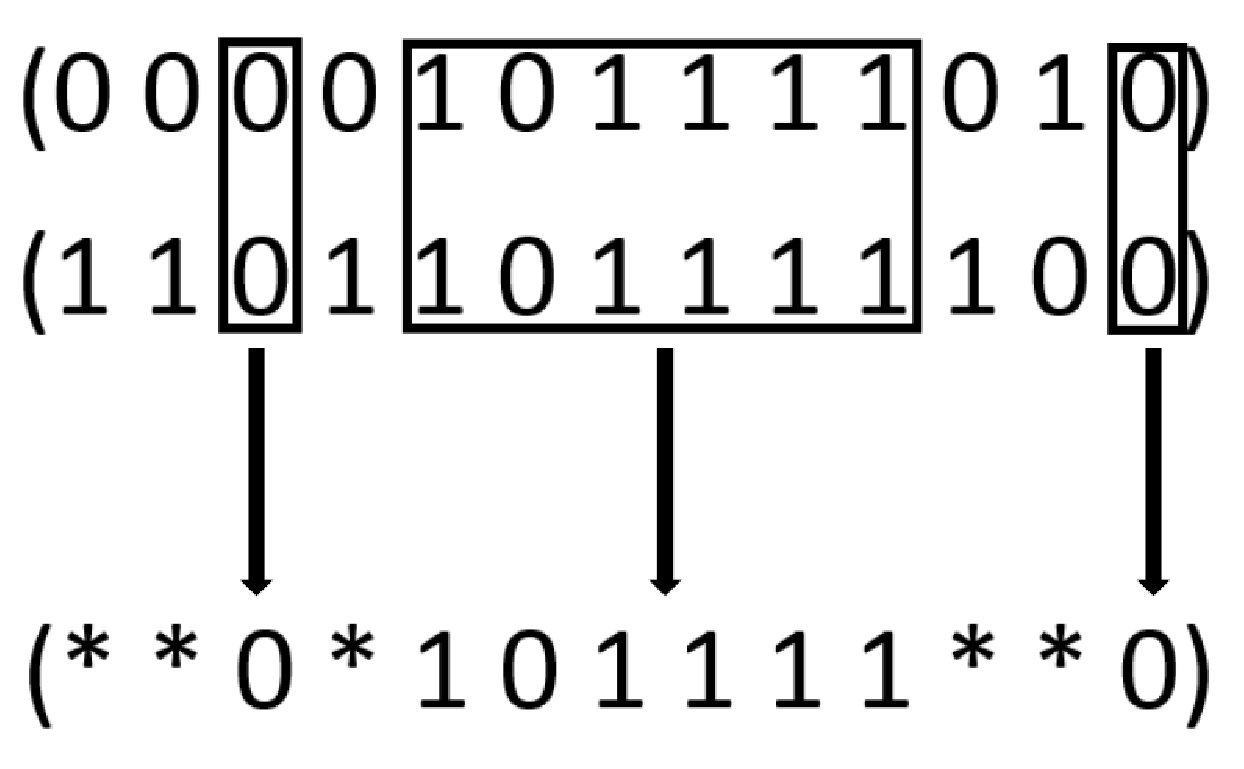
\epsfig{file=crossover.eps,height=2cm,width=4cm}
\end{center}
For each new mutant to be produced, a single parent is selected from the same eugenic pool from the previous generation. 
The newly created mutant also shares many of the characteristics of its parent. 
The mutation function is even simpler : we just switch bits whose locations are randomly chosen
and proportions equal a fixed mutation rate : 
\\\newline
\begin{center}
\textbf{\large Mutation of an individual}
\end{center}
\begin{center}
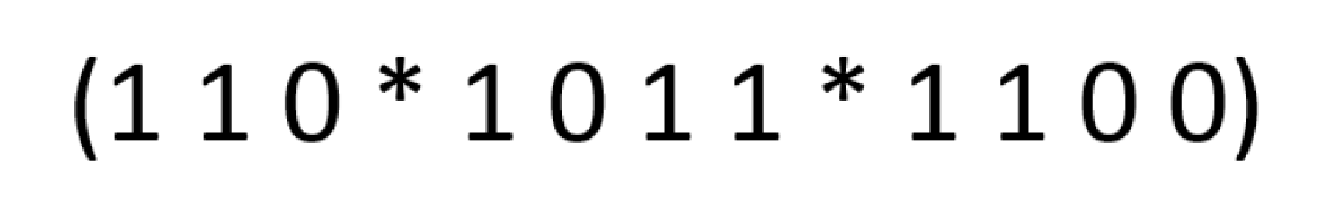
\epsfig{file=mutation.eps,height=0.4cm,width=4cm}
\end{center}
New parents are selected for each new child and mutant, and the process continues until a new population of solutions of appropriate size is generated.
These process ultimately results in the next generation population of chromosomes different from the initial generation. 
Generally the average fitness will have increased by this procedure for the population, 
since only the best organisms from the first generation are selected for breeding and mutating, along with a small proportion of less fit solutions.
These less fit solutions ensure genetic diversity within the genetic pool of the parents and therefore ensure the genetic diversity of the subsequent generation of children.
The number of newly bred fit individuals selected from the current population is a parameter to be fixed, 
The new generation of candidate solutions is then used in the next iteration of the algorithm. 
Commonly, the algorithm terminates when either a maximum number of generations has been produced, or a satisfactory fitness level has been reached for the population.
The evolution usually starts from a population of randomly generated individuals and is an iterative process, with the population in each iteration called a generation.
\\\newline
Let's add here that taking account our mesh constraints is here trivial : we just fix the value of blocs of links between forbidden categories from our
vector. We just end up with a vector with a smaller number of freedom degrees : our adjacency matrix is square but with large fixed null blocks resulting only from locations where links can be added.
\begin{center}
\textbf{\large Links categorization}
\end{center}
\begin{center}
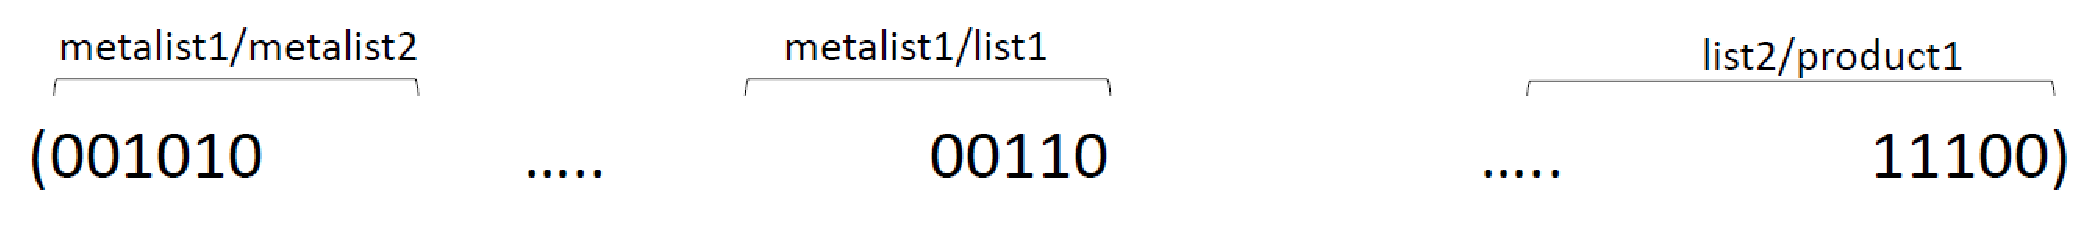
\epsfig{file=links_categorization.eps,height=1cm,width=6cm}
\end{center}
We here present results for a small prototyping use case.
We are provided with 39 URLs. We order and flag them as home, 2 meta lists, 4 lists and 32 products and we affect them
the following vector of importance :
$$
\left(X_i\right)=\{'home','metalist1','metalist2',
$$
$$
'list1','list2','list3','list4',
$$
$$
'product1','product2',...,'product32'\};
$$
$$
f\left(X_i\right) = [100;80;55;$$
$$
40;35;25;20;
$$
$$
4;5;...;3]
$$
Notice that the importance metrics we attribute mirrors the labels we gave. We hope to find back the natural arborescent structure from our algorithm.
Let's now generate our initial population through sheer randomness. Let's visualize it with this picture where x axe represent an individual chromosome, while y runs over all our individuals :
\begin{center}
\textbf{\large Initial population}
\end{center}
\begin{center}
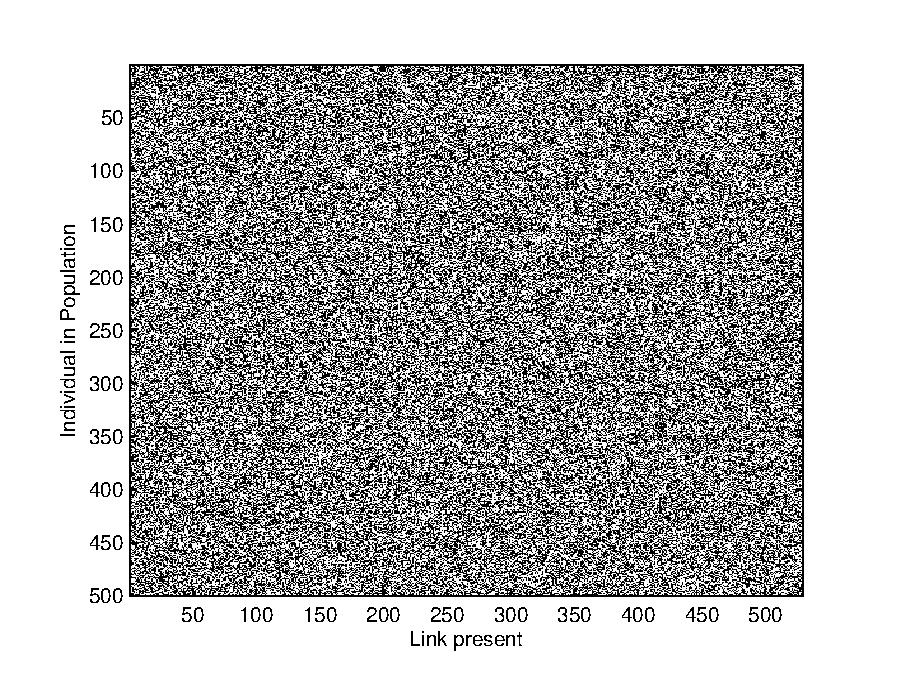
\epsfig{file=initial_population.eps,height=5cm,width=5cm}
\end{center}
For each generation, the fitness of every individual in the population is evaluated. Our fitness function is defined as follows :
First we compute the standard page rank of the individual matching mesh :
The first stage is the page rank initialisation for all our nodes:
\begin{equation}
\forall u \ PR\left(u\right)=\frac{1}{N}
\end{equation} 
We then iterate to find the fixed point solutions of the well know equation :
\begin{equation}
PR\left(u\right)= \frac{\left(1-c\right)}{N} + c \times \sum_{v \rightarrow u}\frac{PR\left(v\right)}{card\left(\left\{v\rightarrow u\right\}\right)}
\end{equation}
The fitness is usually the value of the objective function in the optimization problem being solved.
The fitness function for a mesh $\left(X_i\right)$ is defined as the sum over all nodes of the product of the local importance metrics
and the computed in rank : $\sum^{N}_{i=1} f\left(X_i\right)\times PR(X_i)$, the idea being that by weighing the local importance metrics with the in rank
we'll find the best mesh matching in-rank and the local importance metrics and this for all nodes as the objective is the whole sum. 
So we end up with this generic optimization problem.
\begin{equation}
\max_{\left(G_{ij}\right)  \in \left\{0,1\right\}^{N\times N}}\left\{ \sum^{N}_{i=1} f\left(X_i\right)\times PR(X_i)\right\}
\end{equation}
This is this very same global optimization problem, which can be formulated using different algorithms : simulated annealing, global search, multistart.
Let's here detail the results for our small case toy example of 39 URLs.
For a population of 500 individuals, a mutation rate of $0.2 \%$
Let's here visualize our population at convergence :
\begin{center}
\textbf{\large Population at convergence}
\end{center}
\begin{center}
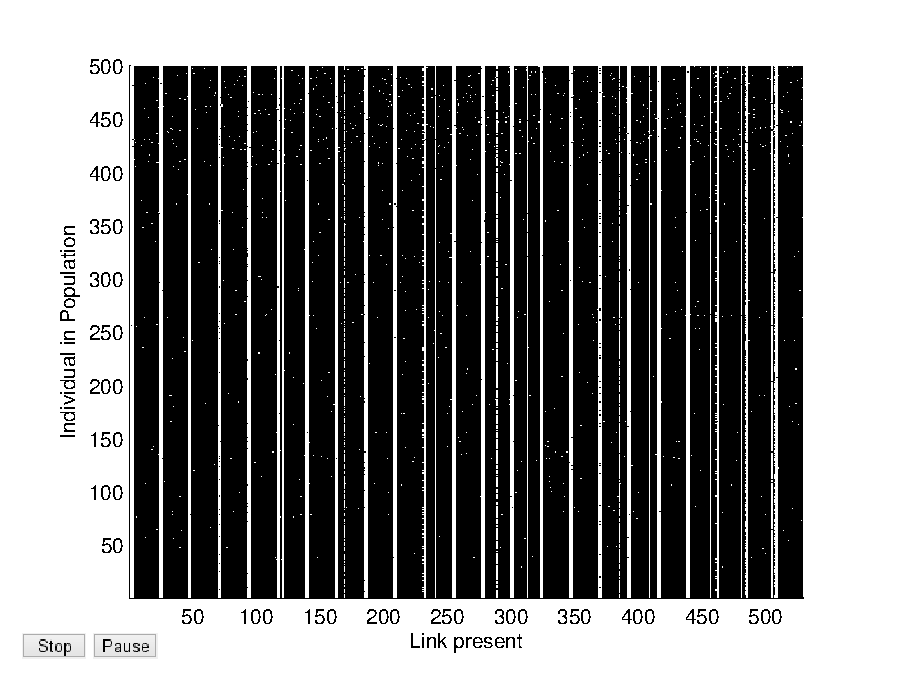
\epsfig{file=converged_population.eps,height=5cm,width=5cm}
\end{center}
\begin{center}
\textbf{\large Best chromosome fitness function evolution}
\end{center}
\begin{center}
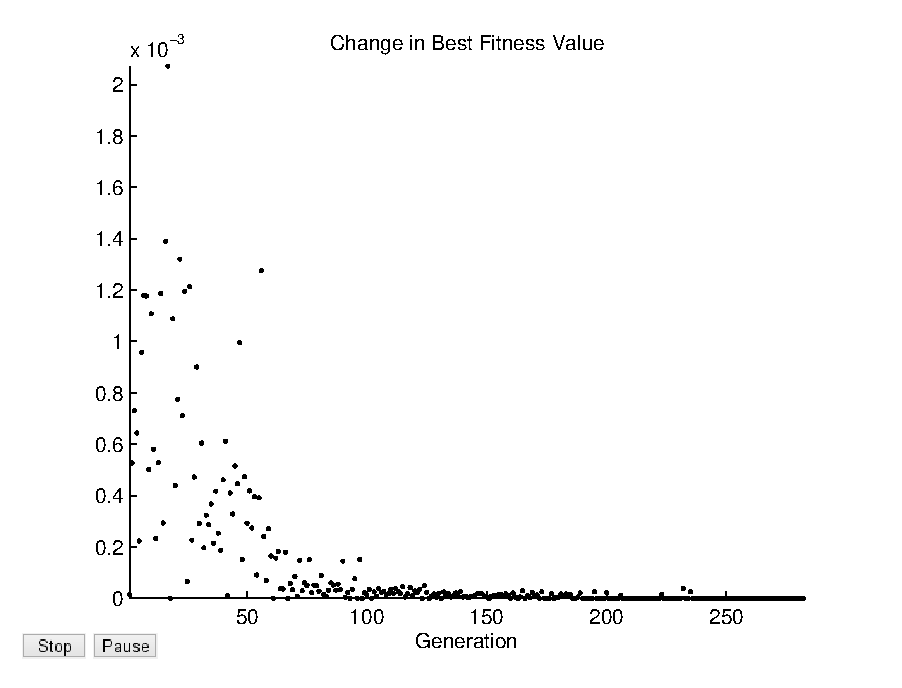
\epsfig{file=best_element_evolution.eps,height=5cm,width=5cm}
\end{center}
\section{An e-commerce approach}
For an e-commerce web site, traffic might not always coincide with the URLs you deem as more profitable to you.
On the very contrary, you may even actually rather want to rebalance some traffic discrepancies.
Of course, the methodology presented above is still valid. You here just have to change the importance vector you want to
optimize. In that case, you would for instance rather optimize $\frac{1}{traffic\left(i\right)}$.
\\\newline
But to get a real sense of potential return on investment, we must here switch to a new paradigm.
Each page will be matched with a specific keywords expression to rank upon. And the potential return on investment for the keywords expression will
be assessed with both search engine data (click through rate, search volume) and e-commerce tracking data (transformation rate).
To push potentially high return on investment pages, we use the following objective function :
\begin{equation}
 \sum_{i\in Keywords} SV\left( i\right)\times CTR\left(position\left(i\right)\right)\times CR\left(i\right)\times P\left(i\right)
\end{equation}
where $position\left(i\right)$ is the estimated position in search engine results coming from the modification of our new mesh,
\\\newline
$SV\left(i\right)$ is the search volume for the keywords $i$ estimated by the search engine.
\\\newline
and $CTR\left(i\right)$ is the click through rate for an URL at the position place in the search engine results.
\\\newline



Page rank thematic little topo here.


\section{Big data implementaion}
The double iterative nature of our algorithm (page rank computations and optimization are both naturally iterative)
makes Hadoop Map/Reduce paradigm too slow for our purpose. 
In contrast to Hadoop's two-stage disk based Map/Reduce paradigm, Spark's in-memory primitives provide the needed performance.
By allowing user programs to load data into a cluster's memory and query it repeatedly, Spark is well suited for our purpose.
We'll detail the technological implementation of a real-world use case.



The in rank fitness function is computed recurrently over the whole population. To improve its performance is key for an efficient
algorithm. The idea here would be to computed an approximated in rank using \cite{}.

The sparsitiy of the matrix has to be addressed.


%\lipsum
%A citation example: \cite{donald1999art}.

\bibliographystyle{plain}
\bibliography{biblio}
\end{document}